\section{\ExercisePrefixEmbeddedC Testprogramm auf den Microcontroller laden \optional}

Alle nun folgenden, mit \ExercisePrefixEmbeddedC markierten Aufgaben sind nicht klausurrelevant.
Sie dienen dazu, dich in die Welt der Embedded-C-Programmierung einzuführen.
Embedded C ist hierbei genau die gleiche Programmiersprache wie C.
Jedoch gibt es einige technische Besonderheiten zu berücksichtigen.

\subsection{Überblick}
Für die Arbeit mit dem Evaluationsboard nutzen wir die Entwicklungsumgebung \emph{WinIDEA Open}\footnote{\url{http://www.isystem.com/download/winideaopen}}.
%
Im Vergleich zu CodeLite ist diese Umgebung speziell auf die Entwicklung von Embedded C zugeschnitten.
Der Bauprozess für Embedded-C-Programme sieht teilweise anders aus als bei C++-Programmen:
\begin{enumerate}
\item 
Das Ergebnis der \textbf{Link-Phase} ist kein auf dem PC ausführbares Programm, sondern ein sogenanntes \emph{Image}.
Dieses Image wird in den statischen Speicher des Microcontrollers geladen.
\item
Nach der Link-Phase folgt die \textbf{Flash-Phase} (in WinIDEA auch \enquote{Download} genannt).
Während dieser Phase wird das Image auf den Microcontroller übertragen.
\item 
Anschließend beginnt die \textbf{Ausführung} direkt oder man muss den \emph{Reset}-Knopf des Boards drücken, um den Programmzähler zurückzusetzen.
\item
Standardmäßig geht WinIDEA hierbei direkt in den \textbf{Debug-Modus}.
Das bedeutet, dass die Ausführung des Programms am Beginn der \lstinline|main|-Funktion angehalten wird.
\end{enumerate}

Die weiteren Besonderheiten vom Embedded C sehen wir uns anhand eines einfachen Testprogramms an.

\subsection{Testprogramm}
Für diese und alle weiteren Aufgaben stellen wir dir ein Codetemplate zur Verfügung, das von dir ergänzt wird.
Wir beginnen mit einem kleinen fertigen Programm, das die RGB-LED des Evaluationsboards periodisch blinken lässt.
Dies ist das \enquote{Hello World}-Programm der Embedded-C-Welt.

\begin{enumerate}
\item 
Kopiere zunächst den \textbf{vorbereiteten WinIDEA-Workspace} (\filename{/exercises/templates/05\_Win\-Idea\-Workspace\-Template}) in ein Verzeichnis \textbf{außerhalb} deines Benutzerverzeichnisses (\bspw nach \filename{C:\textbackslash{}tmp}).
\footnote{Leider ist es aus technischen Gründen nicht möglich, mit WinIDEA im Benutzerverzeichnis zu arbeiten, da dieses auf ein Netzlaufwerk abgebildet wird.}
Falls du deinen eigenen PC verwendest, ist es sehr wichtig, dass der WinIDEA-Workspace und die verwendeten Bibliotheken (bspw. \filename{C:\textbackslash{}PortableApps\textbackslash{}Cypress\textbackslash{}PDL}) auf dem gleichen Laufwerk liegen.

\item 
\textbf{Öffne WinIDEA}:
Das Programm liegt unter \filename{C:\textbackslash{}PortableApps\textbackslash{}iSYSTEM\textbackslash{}winIDEAOpen9\textbackslash{}winIDEA.exe}.
Bei Bedarf kannst du dir eine Desktop-Verknüpfung erstellen.

\item 
\textbf{Wähle} in dem erscheinenden Dialogfenster den soeben \textbf{kopierten WinIDEA-Workspace} aus wie in Abbildung \ref{fig:WinIdeaSelectWorkspace} gezeigt (roter Rahmen).
\begin{figure}
\begin{centering}
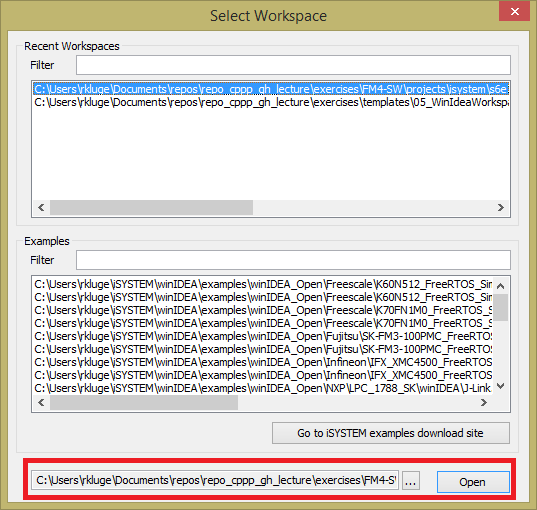
\includegraphics[width=.5\textwidth]{./05_c/figures/WinIDEASelectWorkspace.png}
\caption{Workspace-Auswahl in WinIDEA}
\label{fig:WinIdeaSelectWorkspace}
\end{centering}
\end{figure}

\item 
Nun öffnet sich der eigentliche Workspace.
Du findest links einen baumartig aufgebauten Datei-Browser, der die Datei-Gruppen \winIdeaGroupName{lib}, \winIdeaGroupName{src} und \winIdeaGroupName{Dependencies} enthält.
\begin{itemize}
\item
Die Gruppe \winIdeaGroupName{lib} enthält manuell konfigurierte Abhängigkeiten deines Projekts, die du normalerweise nicht anpassen musst.
\item 
Die Gruppe \winIdeaGroupName{src} enthält den Quelltext, mit dem du arbeiten wirst.
\item 
Die Gruppe \winIdeaGroupName{Dependencies} enthält automatisch von WinIDEA aufgelöste Abhängigkeiten und muss nicht angepasst werden.
\end{itemize}
\textbf{Öffne} nun die Datei \textbf{\filename{main.c}} in der Gruppe \winIdeaGroupName{src}.

\item
Hier findest du die \textbf{\lstinline|main|-Funktion}, deren Inhalt du im Folgenden immer wieder anpassen wirst.
Im Moment delegiert sie an die Funktion \lstinline|BlinkMain|.
Diese ist in der Datei \filename{blink.h} deklariert und in \filename{blink.c} definiert.
\textbf{Öffne} nun die Datei \textbf{\filename{blink.c}}.

\item 
Du findest den folgenden Quelltext (\Cref{lst:Blink}) vor:
\cpppInputListing[frame=tb,caption={\filename{blink.c}},label={lst:Blink},numbers=left]{./05_c/listings/blink.c}

\begin{itemize}
\item 
Zu Beginn werden zwei Pointer auf das \emph{Data Direction Register (DDR)} und das \emph{Port Data Output Register (PDOR)} angelegt, die einen einfachen Zugriff auf die Datenübertragungsrichtung und die Pin-Belegung der blauen LED ermöglichen.

\item 
Anschließend wird der zur LED gehörige Kanal (AN08) auf den digitalen (statt analogen) Modus geschaltet.

\item 
Daraufhin wird der 8.\;Pin des DDR in den Ausgabe-Modus (statt Einlese-Modus) geschaltet und das PDOR wird auf 1 gesetzt, um die LED auszuschalten (\dasheisst die blaue LED ist \enquote{low active}).
Wir zählen Pins immer von 0, \dasheisst es gibt 8 Pins vor dem 8.\;Pin und der höchste Pin je Register ist der 31.\;Pin.
\end{itemize}

\item 
Um das Projekt jetzt zu \textbf{compilieren} und zu \textbf{linken}, wähle im Menü \menuPath{Project} den Befehl \menuPath{Make} (oder drücke \shortcut{F7}).
Dieser Befehl wird -- seinem Namen entsprechend -- nur diejenigen Teile neu kompilieren, die sich seit dem letzten Aufruf verändert haben.
Mit dem Befehl \menuPath{Project \menuSep Rebuild} wird das Projekt von Grund auf neu gebaut.
Der Vorgang sollte im \emph{Output}-Fenster\footnote{Kann über \menuPath{View \menuSep Output} oder \shortcut{Alt+2} geöffnet werden.} mit \texttt{0 Error(s)  0 Warning(s)} enden.

\item 
Um das erzeugte Image auf den Microcontroller zu flashen, verbinde den \textbf{Micro-USB-Anschluss CN2} des Boards mit dem \textbf{Data-USB-Port} des PCs.
Die grüne LED in der Nähe des 2x5-Pin-Multicon-Blocks (CN12) sollte nun dauerhaft leuchten.
Wähle anschließend in WinIDEA \textbf{\menuPath{Debug \menuSep Download}} (oder \shortcut{Ctrl + F3}).


\item 
In WinIDEA wird nun ein \textbf{gelber Pfeil} neben der Signatur der \textbf{\lstinline|main|-Funktion} erscheinen.
Dies deutet an, dass du jetzt auf dem Microcontroller debuggen kannst.
\footnote{Dieses Verhalten lässt sich auch ausschalten: \url{https://github.com/Echtzeitsysteme/tud-cppp/wiki/WorkingWithWinIDEAOpen\#how-can-i-prevent-winidea-from-stopping-at-main-after-downloading}}
Setze die Ausführung einfach fort, indem du \textbf{\menuPath{Debug \menuSep Run Control \menuSep Run}} wählst (oder \shortcut{F5}).
Die blaue LED sollte nun blinken.

\item 
Falls dein Programm einmal \enquote{unsauber} startet oder du es neu starten möchtest, kannst du den Programmzähler mithilfe des \textbf{Reset Buttons} zurücksetzen.
Er befindet sich links oberhalb der MCU und ist auch mit \enquote{Reset} beschriftet.
Ganz in der Nähe befindet sich auch der \textbf{User Button}, den wir im Folgenden noch kennenlernen werden.
\end{enumerate}

\noindent\textbf{Herzlichen Glückwunsch -- du bist nun bereit, selber Hand an die Aufgaben zu legen!}

\subsection{LED bunt blinken lassen}
Als erste eigenständige Aufgabe erweiterst du die Funktion \lstinline|BlinkMain| so, dass abwechselnd alle drei möglichen LEDs angesteuert werden.
Führe dazu die folgenden Schritte aus:
\begin{enumerate}
\item 
Öffne die Dateien Dateien \filename{blinkrainbow.h} und \filename{blinkrainbow.c} (in der Gruppe \winIdeaGroupName{src}).

\item 
Nutze die Dateien \filename{blink.h} und \filename{blink.c} als Ausgangspunkt, um diese Aufgabe zu lösen.
\item
Erweitere nun den Code so, dass du auch auf die Ports der roten und grünen LED zugreifst.
\begin{itemize}
\item 
Je nach angesteuerter LED wirst du den \textbf{Port wechseln} müssen.
Die \textbf{Kennung des Ports} entspricht immer dem letzte Zeichen der entsprechenden Konstante (\zB \lstinline|1| in \lstinline|FM4_GPIO->DD1| oder \lstinline|FM4_GPIO->PDOR1|).

\item 
Die \textbf{Ports und Pins der anderen LEDs} findest du \unteranderem im Abschnitt \enquote{3.1.3 User Button and User LED} des FM4 Starter Kit Guides\footnote{\url{http://www.cypress.com/file/290916/download}}.
Das Format ist dabei immer \lstinline|P[PORT_NUMBER][PIN_NUMBER]|.

\item 
Die Pins der roten und grünen LED sind ebenfalls mit \textbf{A/D-Kanälen} verbunden, die du \textbf{deaktivieren} musst.
Nutze dazu das Schaltbild des Evaluationskits\footnote{\url{http://www.cypress.com/file/290921/download}}.
Auf Seite 2 findest du am unteren Rand die \enquote{RGB LED}.
Davon ausgehend suchst du die entsprechenden Pins am Microcontroller heraus.
Jeder Pin ist dort mit mehreren Funktionsbeschreibungen versehen.
Die A/D-Kanalbezeichnungen beginnen immer mit \enquote{AN}.
Zum Beispiel hat die blaue LED am Microcontroller den Pin 106, der auch als Pin 8 von Port 1 (P18) angesprochen werden kann und mit dem A/D-Kanal 08 (AN08) verknüpft ist.
\end{itemize}
\end{enumerate}

\hints{
\item 
Falls du dir nicht sicher bist, wie du die Maske für einen bestimmten Pin generierst, kann es hilfreich sein, sich zuerst die binäre Darstellung aufzuschreiben und diese dann in die hexadezimale Darstellung zu übertragen.
Beispielsweise würde für die blaue LED (Pin 8) die binäre Maske wie folgt aussehen: \lstinline|0b0000 0001 0000 0000|.
Danach überträgst du jeden Block in das entsprechende hexadezimale Zeichen: \lstinline|0x0100|.


\item 
Für diese und die folgenden Kennenlernaufgaben stellen wir dir Musterlösungen direkt im WinIDEA-Workspace bereit.
Du findest sie in der Gruppe \winIdeaGroupName{solution}.
Beachte, dass die (nicht-statischen) Funktionen der Musterlösung und deren entsprechende Implementierungsdateien stets auf \lstinline|_s| enden, um Namenskonflikte mit den Vorlagefunktionen zu vermeiden.
}